%%\documentclass[handout]{beamer}
%\documentclass[aspectratio=169,13pt]{beamer}

%\newcommand{\dee}{\partial}

\newcommand{\bmat}[1]{\begin{bmatrix} \B{#1}_{11} & \B{#1}_{12} \\ \B{#1}_{21} & \B{#1}_{22}\end{bmatrix}}
\newcommand{\blmat}[1]{\begin{bmatrix} \B{#1}_{11} &  \\ \B{#1}_{21} & \B{#1}_{22}\end{bmatrix}}
\newcommand{\brmat}[1]{\begin{bmatrix} \B{#1}_{11} & \B{#1}_{12} \\ & \B{#1}_{22}\end{bmatrix}}
\newcommand{\bomat}[1]{\begin{bmatrix} {#1}_{11} & \B{#1}_{12} \\ \B{#1}_{21} & \B{\uppercase{#1}}_{22}\end{bmatrix}}
\newcommand{\blomat}[1]{\begin{bmatrix} {#1}_{11} & \\ \B{#1}_{21} & \B{\uppercase{#1}}_{22}\end{bmatrix}}
\newcommand{\bromat}[1]{\begin{bmatrix} {#1}_{11} & \B{#1}_{12} \\  & \B{\uppercase{#1}}_{22}\end{bmatrix}}

\DeclareMathOperator{\vcop}{vec}
\newcommand{\vc}[1]{\vcop\left(#1\right)}
\newcommand{\prm}{\mu}

\newcommand{\fl}{fl}
\newcommand{\asmcond}[1]{\smallskip{\it #1}\smallskip}
\newcommand{\amdcond}[1]{\smallskip{\it #1}\smallskip}
\newcommand{\algcond}[1]{\smallskip{\it #1}\smallskip}
\newcommand{\atsmcond}[1]{{\it #1}}
\newcommand{\atmdcond}[1]{{\it #1}}
\newcommand{\atlgcond}[1]{{\it #1}}
\newcommand{\afillnum}[1]{{\underline{ \ #1\ \ }}}

\mode<presentation>
{
  \usetheme{Malmoe}
}

\usepackage[english]{babel}
%
%\usepackage[latin1]{inputenc}
%
%\usepackage{times}
%\usepackage[T1]{fontenc}
% Or whatever. Note that the encoding and the font should match. If T1
% does not look nice, try deleting the line with the fontenc.

\usepackage{inconsolata}
\usepackage{listings}
\usepackage{bm}
\usefonttheme[onlymath]{serif}
\renewcommand\familydefault{\sfdefault}
\usepackage[sfdefault]{ClearSans} %% option 'sfdefault' activates Clear Sans as the default text font
%\usefonttheme{professionalfonts}

\usepackage{latexsym}
\usepackage{amsmath}
\usepackage{amssymb}
\usepackage{amsfonts}
\usepackage{graphics}
\usepackage{multicol}

\definecolor{darkred}{rgb}{0.8,0.2,0.2}
\newcommand{\coloremph}[1]{\textcolor{darkred}{\emph{#1}}}        % colored italics
\newcommand{\reshape}[2]{o_{#1}(#2)}        % colored italics
\newcommand{\ket}[1]{\lvert #1 \rangle}
\newcommand{\bra}[1]{\langle #1 \vert}
\newcommand{\transp}[2]{{#2}^{\langle  {#1} \rangle }}        % colored italics

% Miscellaneous special math symbols

% Big-oh notation - either Latex's calligraphic O or uppercase math italic O
\newcommand{\BIGOH}{\mathcal{O}}                              % big oh
%\newcommand{\BIGOH}{O}                                       % big oh
\newcommand{\BIGTHETA}{\Theta}                                % big theta

\newcommand{\sfrac}[2]{{#1}/{#2}}

% Various versions of the fraction one-half
% solidus 1/2 for superscripts:
\newcommand{\SHALF}{1/2}                                      % one-half power
% small 1/2 set case in displayed equations:
\newcommand{\HALF}{\mbox{\small $\frac{1}{2}$}}               % small one-half
\newcommand{\THRD}{\mbox{\scriptsize $\frac{1}{3}$}}          % small one-third
\newcommand{\TWOTH}{\mbox{\scriptsize $\frac{2}{3}$}}         % small two-thirds

% Machine epsilon - note that placement of subscript may need adjustment.
%\newcommand{\emach}{\epsilon_{\textrm{\scriptsize mach}}} % machine prec.
\newcommand{\emach}{\epsilon}

\newcommand{\lsapprox}{\cong}                             % least squares approx

% Real numbers - Prefer \mathbb{R} but it requires amsfonts.
%                Latex's calligraphic R will do if amsfonts are unavailable.
%                DO NOT use \Re, which gives old German fraktur R.
\newcommand{\Real}{\mathbb{R}}                                 % real numbers
\newcommand{\Cplx}{\mathbb{C}}                                 % complex numbers
\newcommand{\Poly}{\mathbb{P}}                                 % polynomials
\newcommand{\Float}{\mathbb{F}}                                % fl pt system
% Bold math fonts for vectors and matrices
\renewcommand{\Vec}[1]{\ensuremath{\bm{#1}}}                   % vector
\newcommand{\Mat}[1]{\ensuremath{\bm{#1}}}                     % matrix
\newcommand{\Op}[1]{#1}                              % operator
\newcommand{\loc}[1]{x_{#1}}                              % operator

% Loglike functions set in regular type
\newcommand{\diag}{\mathrm{diag}}                             % diagonal matrix
\newcommand{\cond}{\mathrm{cond}}                             % condition number
\newcommand{\sign}{\mathrm{sign}}                             % sign function
\newcommand{\Span}{\text{span}}                             % span of matrix
%\newcommand{\trace}{\mathrm{trace}}                           % trace of matrix
\DeclareMathOperator*{\trace}{trace}
\newcommand{\tentrace}[3]{\trace_{#1,#2}(#3)}
\renewcommand{\Re}{\mathrm{Re}}                               % real part
\renewcommand{\Im}{\mathrm{Im}}                               % imaginary part

% Fractions appearing in matrices - allows setting them case or solidus
%\newcommand{\mf}[2]{{#1 \over #2}}        % matrix fraction - set case
\newcommand{\mf}[2]{#1/#2}               % matrix fraction - set solidus


% Keywords for algorithm statements

\newcommand{\FOR}{\textbf{for}\ }
\newcommand{\TO}{\textbf{to}\ }
\newcommand{\IF}{\textbf{if}\ }
\newcommand{\THEN}{\textbf{then}\ }
\newcommand{\ELSE}{\textbf{else}\ }
\newcommand{\WHILE}{\textbf{while}\ }
\newcommand{\DO}{\textbf{do}\ }
\newcommand{\BEGIN}{\textbf{begin}\ }
\newcommand{\END}{\textbf{end}\ }
\newcommand{\STOP}{\textbf{stop}\ }
\newcommand{\AND}{\textbf{and}\ }
\newcommand{\OR}{\textbf{or}\ }

\newcommand{\comm}{\mathrm{comm}}
\newcommand{\comp}{\mathrm{comp}}
\newcommand{\idle}{\mathrm{idle}}
\newcommand{\msg}{\mathrm{msg}}
\newcommand{\len}{\mathrm{s}}
\newcommand{\route}{\mathrm{route}}
\newcommand{\mitem}{\medskip\item}
\newcommand{\sitem}{\smallskip\item}
\DeclareMathOperator*{\argmin}{argmin}

%Gets rid of headline

\setbeamertemplate{footline}{}

\setbeamertemplate{headline}{}
\beamertemplatenavigationsymbolsempty



\definecolor{mygreen}{rgb}{0,0.2,0}
\definecolor{mygray}{rgb}{0.5,0.5,0.5}
\definecolor{mymauve}{rgb}{0.58,0,0.82}
\definecolor{mypurple}{rgb}{0.38,0,0.32}
\definecolor{myblue}{rgb}{0.2,0,0.5}
\definecolor{darkgreen}{rgb}{0.2,0.6,0.2}
\definecolor{Brown}{rgb}{0.39, 0.09, 0.0}
\definecolor{Violet}{rgb}{0.38, 0.0, 0.63}
\definecolor{myvlgray}{rgb}{0.9,0.9,1.0}
\definecolor{mylgray}{rgb}{0.85,0.85,0.9}
\definecolor{darkgreen}{rgb}{0,0.4,0}
\definecolor{brown}{rgb}{.6,.1,.1}

\newcommand{\bemph}[1]{{\color{blue} \emph{#1}}}

\usepackage{mathtools}
\newcommand{\defeq}{\coloneqq}

\newcommand{\inti}[2]{[{#1},{#2}]}
\newcommand{\BF}{\mathbf}
\newcommand{\CF}{\mathcal}
\newcommand{\B}[1]{\bm{#1}}
\newcommand{\E}[1]{\bm{#1}}
\newcommand{\dis}{\displaystyle}
\newcommand{\lt}{\left}
\newcommand{\rt}{\right}

\newcommand{\cs}{H}

\DeclareMathOperator*{\rank}{rank}
\DeclareMathOperator*{\vecn}{vec}
\DeclareMathOperator*{\vecs}{vech}

\usepackage{eso-pic}
\newcommand{\cornertext}[1]{
  \AddToShipoutPictureFG*{
    \AtPageUpperLeft{\put(0,-10){\makebox[\paperwidth][r]{#1}}}  
   }%
}
\newcommand{\cornertexttwo}[2]{
  \AddToShipoutPictureFG*{
    \AtPageUpperLeft{\put(0,-10){\makebox[\paperwidth][r]{#1}}}  
    \AtPageUpperLeft{\put(0,-20){\makebox[\paperwidth][r]{#2}}}  
   }%
}
\newcommand{\linkdemo}[2]{{\footnotesize\href{https://relate.cs.illinois.edu/course/cs450-f18/f/demos/upload/#1/#2.html}{\color{Violet}{\it\textbf{Demo:} #2}\ }}}
\newcommand{\linkinclass}[2]{{\footnotesize\href{https://relate.cs.illinois.edu/course/cs450-f18/flow/#1/start/}{\color{darkgreen}{\it\textbf{Activity:} #2}\ }}}
\newcommand{\urcornerlinkinclass}[2]{\cornertext{\linkinclass{#1}{#2}}}
\newcommand{\dblurcornerlinkinclass}[4]{\cornertexttwo{\linkinclass{#1}{#2}}{\linkinclass{#3}{#4}}}
\newcommand{\urcornerlinkdemo}[2]{\cornertext{\linkdemo{#1}{#2}}}
\newcommand{\dblurcornerlinkdemo}[4]{\cornertexttwo{\linkdemo{#1}{#2}}{\linkdemo{#3}{#4}}}
\newcommand{\urcornerlinkdemoinclass}[4]{\cornertexttwo{\linkdemo{#1}{#2}}{\linkinclass{#3}{#4}}}



% CS 554 specific:

\newcommand{\tsync}{\alpha}
\newcommand{\tword}{\beta}
\newcommand{\tflop}{\gamma}

\newcommand{\bw}{w}

\newcommand{\tpl}[2]{{\bm{#1}}}
\newcommand{\vtpl}[3]{{\bm{#1}}_#3}
\newcommand{\perm}[2]{\lt[#1\rt]_{#2}}
\newcommand{\costyle}{\ttfamily\bfseries}
\newcommand{\cotext}[1]{{\costyle{#1}}}
\newcommand{\kwstyle}{\costyle\textcolor{mypurple}}
\newcommand{\kwtext}[1]{{\kwstyle{#1}}}
\newcommand{\emstyle}{\costyle\textcolor{myblue}}
\newcommand{\emtext}[1]{{\emstyle{#1}}}
\newcommand{\const}{}
\newcommand{\work}{Q}
\newcommand{\depth}{D}
\newcommand{\flops}{F}
\newcommand{\words}{W}
\newcommand{\syncs}{S}
\newcommand{\mem}{M}
\newcommand{\eff}{E}
\newcommand{\isofun}[1]{\tilde{\work}(p)}
\newcommand{\isomem}[1]{\tilde{\mem}(p)}
\newcommand{\pstrong}{p_s}
\newcommand{\pweak}{p_w}
\newcommand{\ALL}{\star }
\newcommand{\rmn}[2]{\mathbb{R}^{#1\times #2}}
\newcommand{\rn}[1]{\mathbb{R}^{#1}}
\newcommand{\err}{\varepsilon}
\newcommand{\mat}[1]{\begin{bmatrix} #1 \end{bmatrix}}
\newcommand{\mc}[1]{\mathcal{#1}}
\newcommand{\h}[2]{\mc{H}_{#1}(#2)}
\newcommand{\T}{T}%{\mathsf{T}}
\newcommand{\dn}[2]{\mc{M}_{#1}^{\uparrow}(#2)}
%\usepackage[colorlinks=false,urlbordercolor={1.0 1.0 1.0}]{hyperref}
%
%\lstset{ %
%  postbreak=false,
%%  backgroundcolor=\color{white},   % choose the background color; you must add \usepackage{color} or \usepackage{xcolor}
%  basicstyle=\costyle,        % the size of the fonts that are used for the code
%%  breakatwhitespace=false,         % sets if automatic breaks should only happen at whitespace
%%  breaklines=false,                 % sets automatic line breaking
%  captionpos=n,                    % sets the caption-position to bottom
%  commentstyle=\color{mygreen},    % comment style
%  deletekeywords={...},            % if you want to delete keywords from the given language
%  escapeinside={\%*}{*)},          % if you want to add LaTeX within your code
%  extendedchars=true,              % lets you use non-ASCII characters; for 8-bits encodings only, does not work with UTF-8
%  frame=none,                    % adds a frame around the code
%  keepspaces=true,                 % keeps spaces in text, useful for keeping indentation of code (possibly needs columns=flexible)
%  keywordstyle=\color{mypurple},       % keyword style
%  language=C++,                 % the language of the code
%  otherkeywords={*,...},            % if you want to add more keywords to the set
%  numbers=none,                    % where to put the line-numbers; possible values are (none, left, right)
%  numbersep=5pt,                   % how far the line-numbers are from the code
%  numberstyle=\tiny\color{mygray}, % the style that is used for the line-numbers
%  rulecolor=\color{black},         % if not set, the frame-color may be changed on line-breaks within not-black text (e.g. comments (green here))
%  showspaces=false,                % show spaces everywhere adding particular underscores; it overrides 'showstringspaces'
%  showstringspaces=false,          % underline spaces within strings only
%  showtabs=false,                  % show tabs within strings adding particular underscores
%  stepnumber=2,                    % the step between two line-numbers. If it's 1, each line will be numbered
%  stringstyle=\color{mymauve},     % string literal style
%  tabsize=2,                     % sets default tabsize to 2 spaces
%  title=\lstname,                   % show the filename of files included with \lstinputlisting; also try caption instead of title
%  keywordstyle=\emstyle
%}

\lstset{ %
  postbreak=false,
%  backgroundcolor=\color{white},   % choose the background color; you must add \usepackage{color} or \usepackage{xcolor}
  basicstyle=\footnotesize\costyle,        % the size of the fonts that are used for the code
%  breakatwhitespace=false,         % sets if automatic breaks should only happen at whitespace
%  breaklines=false,                 % sets automatic line breaking
  captionpos=n,                    % sets the caption-position to bottom
  commentstyle=\color{mygreen},    % comment style
  deletekeywords={privatei,shared},            % if you want to delete keywords from the given language
  escapeinside={\%*}{*)},          % if you want to add LaTeX within your code
  extendedchars=true,              % lets you use non-ASCII characters; for 8-bits encodings only, does not work with UTF-8
  frame=none,                    % adds a frame around the code
  keepspaces=true,                 % keeps spaces in text, useful for keeping indentation of code (possibly needs columns=flexible)
  keywordstyle=\footnotesize\color{mypurple},       % keyword style
  language=C++,                 % the language of the code
  otherkeywords={*,pragma},            % if you want to add more keywords to the set
  numbers=none,                    % where to put the line-numbers; possible values are (none, left, right)
  numbersep=5pt,                   % how far the line-numbers are from the code
  numberstyle=\footnotesize\color{mygray}, % the style that is used for the line-numbers
  rulecolor=\color{black},         % if not set, the frame-color may be changed on line-breaks within not-black text (e.g. comments (green here))
  showspaces=false,                % show spaces everywhere adding particular underscores; it overrides 'showstringspaces'
  showstringspaces=false,          % underline spaces within strings only
  showtabs=false,                  % show tabs within strings adding particular underscores
  stepnumber=2,                    % the step between two line-numbers. If it's 1, each line will be numbered
  stringstyle=\footnotesize\color{mymauve},     % string literal style
  tabsize=2,                     % sets default tabsize to 2 spaces
  title=\lstname,                   % show the filename of files included with \lstinputlisting; also try caption instead of title
  emph={MPI_Send,MPI_Recv,MPI_Comm,MPI_Comm_rank,MPI_Send,MPI_Comm_split,MPI_Init,MPI_Finalize,MPI_Status,MPI_COMM_WORLD,MPI_Datatype,MPI_Comm_size,MPI_FLOAT,mpi.h,omp,parallel,shared,private,default,reduction},
  emphstyle=\footnotesize\emstyle
}

\title{CS 450: Numerical Anlaysis\footnote{{\it These slides have been drafted by Edgar Solomonik as lecture templates and supplementary material for the book ``Scientific Computing: An Introductory Survey'' by Michael T. Heath (\href{http://heath.cs.illinois.edu/scicomp/notes/index.html}{{\color{blue} slides}}).}}}
\author{}
\institute{University of Illinois at Urbana-Champaign}




\subtitle{Interpolation}

\date{}
\begin{document}

\begin{frame}
  \titlepage
\end{frame}

\section{Interpolation and Vandermonde Systems}

\begin{frame}{Interpolation}

\begin{itemize}
\item Given $(t_1,y_1),\ldots ,(t_m,y_m)$ with \coloremph{nodes} $t_1<\cdots < t_m$ an \coloremph{interpolant} $f$ satisfies:

\lgcond{
   \[f(t_i)=y_i \quad \forall i.\]

\begin{itemize}
\item The number of possible interpolant functions is infinite, but there is a unique degree $m-1$ polynomial interpolant.
\sitem Error of interpolant can be quantified with knowledge of true function $g$, (e.g. by considering $\max_{t\in[t_1,t_m]} |f(t)-g(t)|$) .
\end{itemize}
}

\item Interpolant is usually constructed as linear combinations of \coloremph{basis functions} $\{\phi_j\}_{j=1}^n=\phi_1,\ldots,\phi_n$ so $f(t)=\sum_j x_j\phi_j(t)$.


\lgcond{
\begin{itemize}
\sitem Interpolant exists if $n \geq m$ and is unique for a given basis if $n=m$.
\mitem \coloremph{Vandermonde matrix} $\B A = \B V(\B t,\{\phi_j\}_{j=1}^n)$ satisfies $a_{ij}=\phi_j(t_i)$ so $\B A \B x = \B y$.
\mitem Coefficients $\B x$ of interpolant are obtained by solving \coloremph{Vandermonde system} $\B A\B x =\B y$ for $\B x$.
%\sitem Interpolant can be evaluated at any point $t$ by computing $y=\B V(\B t,\{\phi_j\}_{j=1}^n)$ then $\B y=\B B \B x$.
\end{itemize}
}

\end{itemize}


\end{frame}


\begin{frame}{Polynomial Interpolation}

\urcornerlinkinclass{inclass-interpolation-monomial}{Interpolation in Monomial Basis}

\begin{itemize}
\item The choice of \coloremph{monomials} as basis functions, $\phi_j(t)=t^{j-1}$ yields a degree $n-1$ polynomial interpolant:


\lgcond{
\begin{itemize}
\sitem Corresponding Vandermonde matrix $\B A = \B V(\B t, \{t^{j-1}\}_{j=1}^n)$ satisfies $a_{ij}=t_i^{j-1}$.
\end{itemize}
}

\item Polynomial interpolants are easy to evaluate and do calculus on:
%They are easy to differentiate, integrate, and evaluate, e.g. via Horner's rule
\lgcond{
\begin{itemize} 
\sitem \coloremph{Horner's rule} requires $n$ products and $n-1$ additions:
  \[f(t) = x_1 + t(x_2 + t(x_3 +\ldots )).\]
\item $O(n)$ work to determine new coefficients for differentiation and integration.
\end{itemize}
}

\end{itemize}

\end{frame}

%\begin{frame}{Solving a Vandermonde System}
%
%\begin{itemize}
%\item Naively, polynomial interpolation requires $O(n^3)$ work for solving the linear system $\B A \B x = \B y$:
%
%\mdcond{
%Gaussian elimination of $\B A$ requires $O(n^3)$ work.
%By comparison evaluating the polynomial is only $O(n)$ work.
%}
%
%\item 
%Polynomial interpolants are easy to evaluate and do calculus on:
%They are easy to differentiate, integrate, and evaluate, e.g. via Horner's rule
%\lgcond{
%  \[f(t) = x_1 + t(x_2 + t(x_3 +\ldots ))\]
%\begin{itemize} 
%\item Differentiation and integration require $m$ products.
%\mitem Horner's rule for evaluation requires $m$ products and $m$ additions
%\end{itemize}
%}
%
%\end{itemize}
%
%\end{frame}


\section{Conditioning of Interpolation}

\begin{frame}{Conditioning of Interpolation}

\urcornerlinkdemo{07-interpolation}{Monomial interpolation}

\begin{itemize}
\item Conditioning of interpolation matrix $\B A$ depends on basis functions and coordinates $t_1,\ldots, t_m$:

\lgcond{
\begin{itemize}
\item $t_i$ defines the $i$th row, so columns tend to be nearly linearly-dependent if $t_i\approx t_{i+1}$
\sitem $\phi_j$ defines the $j$th column, so rows tend to be nearly linearly-dependent if $\phi_j$ is nearly in the span of the other basis functions: $\mathop{span}(\{\phi_i\}_{i=1,i\neq j}^n)$
\end{itemize}
}

\item The Vandermonde matrix tends to be ill-conditioned:
\lgcond{
\begin{itemize} 
\item Monomials of increasing degree increasingly resemble one-another, so rows of $\B A$ become nearly the same, and consequently $\kappa(\B A)$ grows.
\mitem The conditioning can be improved somewhat by shifting and scaling points so that each $t_i\in [-1,1]$.
\mitem Consequently, we will consider alternative polynomial bases, seeking to improve the efficiency and conditioning associated with the Vandermonde matrix.
\mitem However, generally, we will obtain the {\it same} polynomial interpolant. To improve interpolant quality (e.g. avoid oscillations), the nodes and not the basis functions need to be changed.
\end{itemize}
}

\end{itemize}


\end{frame}

\section{Efficient Bases}

\begin{frame}{Lagrange Basis}

\begin{itemize}
\item $n$-points fully define the unique $(n-1)$-degree polynomial interpolant in the \coloremph{Lagrange basis}:
\lgcond{
\[\phi_j(t) = \underbrace{\prod_{k=1,k\neq j}^n (t-t_k)}_{\textbf{num}}/\underbrace{\prod_{k=1,k\neq j}^n (t_j-t_k)}_{\textbf{den}}\]
\begin{itemize}
\item Note that \textbf{den} is never $0$,
\sitem \textbf{num} is $0$ whenever $t=t_k$ for some $k$, so $\phi_j(t_i)=0$ if $i \neq j$,
\sitem when $t=t_j$ then \textbf{num} and \textbf{dem} are the same, so $\phi_j(t_j)=1$,
\sitem consequently, the Lagrange Vandermonde matrix $\B V(\B t, \{\phi_j\}_{j=1}^n) = \B I$.
\end{itemize}
}

\item Lagrange polynomials yield an ideal Vandermonde system, but the basis functions are hard to evaluate and do calculus on:
\lgcond{
\begin{itemize} 
\item Evaluation requires $O(n^2)$ work naively and may incur cancellation error.
\mitem Differentiation and integration are also harder than with monomials.
\end{itemize}
}

\end{itemize}

\end{frame}


\begin{frame}{Newton Basis}

\begin{itemize}
\item The \coloremph{Newton basis} functions $\phi_j(t) = \prod_{k=1}^{j-1}(t-t_k)$ with $\phi_1(t)=1$ seek the best of monomial and Lagrange bases:

\lgcond{
\begin{itemize}
\sitem Evaluation with Newton basis can use recurrence,
\[\phi_j(t) = \phi_{j-1}(t)(t-t_j).\]
\item Divided difference recurrence enables fast computation of coefficients.
\end{itemize}
}

\item The Newton basis yields a triangular Vandermonde system:

\lgcond{
\begin{itemize}
\sitem Note that $a_{ij}=\phi_j(t_i)=0$ for all $i<j$, so $\B A$ is lower-triangular. 
\mitem Given $\B A$, can use back-substitution to obtain the solution in $O(n^2)$ work.
\mitem Can use evaluation recurrence to compute $\B A$ with $O(n^2)$ work, but divided difference recurrence is more stable than forming $\B A$.
\end{itemize}
}


\end{itemize}

\end{frame}

%\begin{frame}{Recurrences for Newton Basis}
%
%\begin{itemize}
%\item The Newton basis functions $\phi_j(t) = \prod_{k=1}^{j-1}(t-t_k)$ can be evaluated at $t$ with $O(n)$ work using a simple recurrence:
%
%\mdcond{
%\[\phi_j(t) = \phi_{j-1}(t)(t-t_j)\]
%}
%
%\item A recurrence known as the divided-differences formula gives a stable way of efficiently computing the coefficients $\B x$:
%
%\lgcond{
%\[x_i = l_{i1} \quad \text{where} \quad l_{ij}=\frac{l_{i,j+1} - l_{i-1,j}}{t_i-t_{j}} \ \text{for} \ i>j \quad \text{and} \quad l_{ii}= y_i\]
%\begin{itemize}
%\item We can define $x_i=l_{i1}=f[t_1,\ldots, t_i]$ and generally $l_{ij}=f[t_j,\ldots, t_i]$.
%\mitem This recurrence also implies that the Newton coefficients can be constructed incrementally by appending new rows to the bottom of $\B L$.
%\end{itemize}
%}
%\mdcond{}
%
%\end{itemize}
%
%\end{frame}
\section{Orthogonal Polynomials}

\begin{frame}{Orthogonal Polynomials}


\begin{itemize}
\item Recall that good conditioning for interpolation is achieved by constructing a well-conditioned Vandermonde matrix, which is the case when the columns (corresponding to each basis
function) are orthonormal. To construct robust basis sets, we introduce a notion of \coloremph{orthonormal functions}:

\lgcond{
\begin{itemize}
\sitem To compute overlap between basis functions, use a $w$-weighted integral as inner product,
\[\langle p, q\rangle_w = \int_{-\infty}^{\infty} p(t)q(t)w(t) dt.\]
\item $\{\phi_i\}_{i=1}^n$ are orthonormal with respect to the above inner product if
\[\langle \phi_i, \phi_j\rangle_w =\delta_{ij}= \begin{cases} 1 & \text{if} \ i=j \\ 0 & \text{otherwise} \end{cases}. \]
\item The corresponding norm is given by $||f|| = \sqrt{\langle f, f\rangle_w}$.
\end{itemize}
}
\lgcond{
}

\end{itemize}

\end{frame}

\begin{frame}{Legendre Polynomials}

\urcornerlinkdemo{07-interpolation}{Orthogonal Polynomials}

\begin{itemize}
\item The Gram-Schmidt orthogonalization procedure can be used to obtain an orthonormal basis with the same span as any given arbitrary basis:

\lgcond{
Given orthonormal functions $\{\hat{\phi}_i\}_{i=1}^{k-1}$ obtain $k$th function from $\phi_k$ via
\[\hat{\phi}_k(t) = \frac{\hat{\psi}_k(t)}{||{\hat{\psi}_k}||}, \quad \psi_k(t)= \phi_k(t) - \sum_{i=1}^{k-1} \langle \phi_k(t), \hat{\phi}_i(t)\rangle_w \hat{\phi}_i(t)\]
}
\item The \coloremph{Legendre polynomials} are obtained by Gram-Schmidt on the monomial basis, with
$w(t)=\begin{cases} 1 : -1 \leq t \leq 1 \\ 0 : \text{otherwise} \end{cases}$ and normalized so $\hat{\phi}_i(1)=1$.

\lgcond{
For example, $\{\hat{\phi}_i(t)\}_{i=1}^{3}=\{1,t,(3t^2-1)/2\}$ since
\begin{align*}
\psi_1(t) &= 1, \quad
\psi_2(t) = t - \frac{1}{2}\int_{-1}^1 t dt= t \\
\psi_3(t) &= t^2 - \frac{1}{2}\int_{-1}^1 t^2 dt - t \int_{-1}^1 t^3 dt   = t^2 - 1/3 
\end{align*}
}

\end{itemize}

\end{frame}

%\begin{frame}{Basis Orthogonality and Conditioning}
%
%\begin{itemize}
%\item To obtain perfectly conditioned Vandermonde system, want inner products of different columns to be zero:
%
%\lgcond{
%\[\langle \B{a}_i, \B{a}_j \rangle = \sum_{k=1}^n \phi_i(t_k)\phi_j(t_k) = \delta_{ij}\]
%}
%
%\item These inner products should be close to zero, if they are a suitable quadrature rule for our weighted functional inner product:
%
%\lgcond{
%\[\sum_{k=1}^n \phi_i(t_k)\phi_j(t_k) \approx \int_{-\infty}^{\infty} w(t) \phi_i(t)\phi_j(t) dt\]
%For example above holds as equality if we choose
%\[w(t) = \begin{cases} \infty & : t = t_k \ \text{for some} \  k \\ 0 & : \text{otherwise}\end{cases} \]
%}
%
%\end{itemize}
%
%\end{frame}

\section{Chebyshev Interpolation}

\begin{frame}{Chebyshev Basis}

\urcornerlinkdemoinclass{07-interpolation}{Chebyshev interpolation}{inclass-chebyshev}{Chebyshev Interpolation}

\begin{itemize}
\item \coloremph{Chebyshev polynomials} $\phi_j(t) = \cos((j-1) \arccos(t))$ and \coloremph{Chebyshev nodes} $t_i = \cos\left(\frac{2i-1}{2n}\pi\right)$ provide a way to pick \coloremph{nodes} $t_1,\ldots, t_n$ along with a basis, to yield perfect conditioning:

\lgcond{
\begin{itemize}
\item They satisfy the recurrence $\phi_1(t)=1, \phi_2(t)=t, \phi_{i+1}(t) = 2t\phi_i(t)-\phi_{i-1}(t)$
\sitem The Chebyshev basis functions are orthonormal with respect to 
\[w(t)=\begin{cases} 1/(1-t^2)^{1/2} &: -1 \leq t \leq 1 \\ 0 &: \text{otherwise} \end{cases}.\]
\item The Chebyshev nodes ensure orthogonality of the columns of $\B A$, since
\begin{align*}
\sum_{k=1}^n \phi_l(t_k)\phi_j(t_k) &= \sum_{k=1}^n \cos\left(\frac{(l-1)(2k-1)}{2n}\pi\right)\cos\left(\frac{(j-1)(2k-1)}{2n}\pi\right) 
%&=2\sum_{k=1}^n e^{i\frac{(l-j)(2k-1)}{2n}\pi}=\begin{cases} 2 : l=j \\ 0 : \text{otherwise}\end{cases}
\end{align*}
is zero whenever $j\neq l$ due to periodicity of the summands.
\end{itemize}
}
\lgcond{}
\end{itemize}

\end{frame}


\begin{frame}{Chebyshev Nodes Intuition}

\urcornerlinkdemo{07-interpolation}{Jump with Chebyshev Nodes}

{

\centering
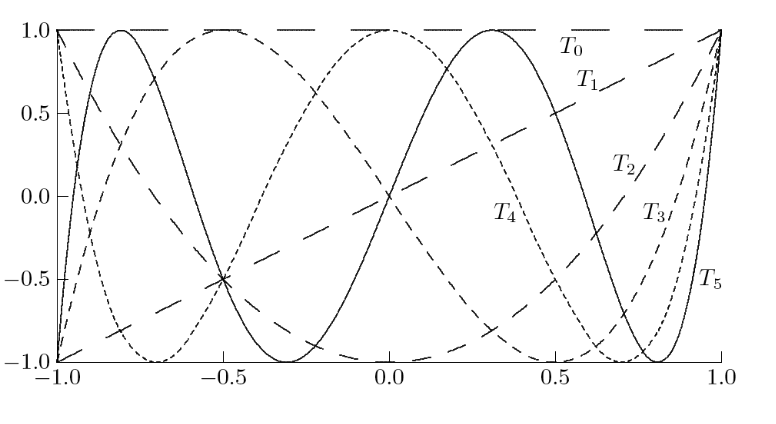
\includegraphics[width=2.4in]{diagrams/cheb_funs}
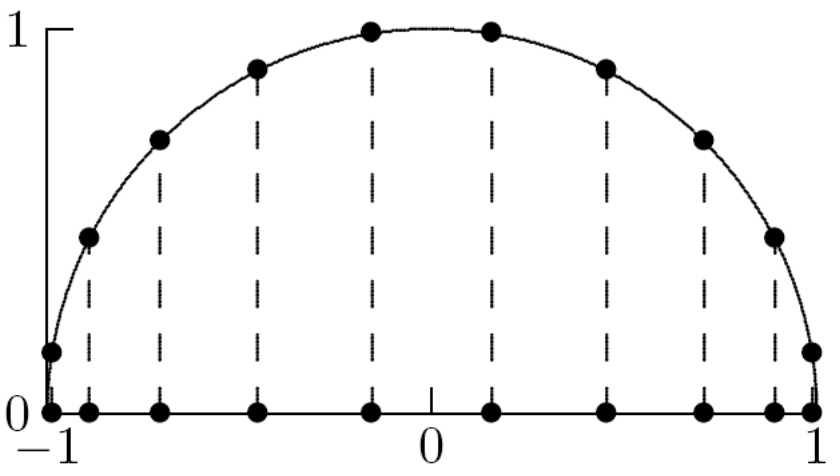
\includegraphics[width=2.2in]{diagrams/chebyshev_nodes}

}
\begin{itemize}
\mitem Note \coloremph{equi-oscillation} property, successive extrema of $T_k=\phi_k$ have the same magnitude but opposite sign.

%\mdcond{}

\mitem Set of $k$ Chebyshev nodes of are given by zeros of $T_k$ and are abscissas of points uniformly spaced on the unit circle.

%\mdcond{}
\end{itemize}

\end{frame}



%\begin{frame}{Orthogonal Polynomials and Recurrences}
%
%\begin{itemize}
%
%\sitem The Newton polynomials could be obtained by a two-term recurrence
%
%\mitem Legendre and Chebyshev polynomials also satisfy three-term recurrence, for Chebyshev
%\[\phi_{i+1}(t) = 2t\phi_i(t)-\phi_{i-1}(t)\]
%
%\mitem In fact all orthogonal polynomials satisfy some recurrence of the form,
%
%\lgcond{
%\[\phi_{i+1}(t) = (\alpha_kt+\beta_k)\phi_i(t)-\gamma_k \phi_{i-1}(t)\]
%
%}
%
%\end{itemize}
%
%
%\end{frame}
\section{Error in Interpolation}

%\begin{frame}{Error in Interpolation}
%
%
%Given degree $2$ polynomial interpolant $\tilde{f}$ the error $E(t)=f(t)-\tilde{f}(t)$ has $2$ zeros at the nodes $t_1,\ldots, t_{2}$ and there exist $y_1, y_2$ such that
%\begin{align}
%E(t) &= \int_{t_1}^t \int_{y_1}^{w_0}\int_{y_2}^{w_1} f'''(w_1) dw_1  dw_0 dy_1 \label{eq:interp_ind}
%\end{align}
%\lgcond{
%\begin{align}
%E(t) &= E(t_1) + \int_{t_1}^t E'(w_0)  dw_0  \label{eq:interp_exp}
%\end{align}
%Now note that for each of $n-1$ consecutive pairs $t_i$, $t_{i+1}$ we have
%\[\int_{t_i}^{t_{i+1}} E'(t) dt = E(t_{i+1})-E(t_i) =  0\]
%and so there are $z_i\in (t_i,t_{i+1})$ such that $E'(z_i)=0$.
%By inductive hypothesis
%\begin{align}
%E'(w_0) &= \int_{z_1}^{w_0} \int_{y_2}^{w_1}\cdots \int_{y_{n}}^{w_{n-1}} f^{(n+1)}(w_n) dw_n \cdots  dw_1  \label{eq:interp_drv}
%\end{align}
%Substituting \eqref{eq:interp_drv} into \eqref{eq:interp_exp}, we obtain \eqref{eq:interp_ind} with $y_1=z_1$.
%}
%\lgcond{
%}
%\end{frame}
%

\begin{frame}{Error in Interpolation}


We show by induction that given degree $n$ polynomial interpolant $\tilde{f}$ of $f$ the error $E(t)=f(t)-\tilde{f}(t)$ has $n$ zeros $t_1,\ldots, t_{n}$ and there exist $y_1,\ldots, y_n$ so
\begin{align}
E(t) &= \int_{t_1}^t \int_{y_1}^{w_0}\cdots \int_{y_n}^{w_{n-1}} f^{(n+1)}(w_n) dw_n \cdots  dw_0 \label{eq:interp_ind}
\end{align}
\lgcond{
\vspace{-.1in}
\begin{align}
E(t) &= E(t_1) + \int_{t_1}^t E'(w_0)  dw_0  \label{eq:interp_exp}
\end{align}
Now note that for each of $n-1$ consecutive pairs $t_i$, $t_{i+1}$ we have
\[\int_{t_i}^{t_{i+1}} E'(t) dt = E(t_{i+1})-E(t_i) =  0\]
and so there are $n-1$ zeros $z_i\in (t_i,t_{i+1})$ such that $E'(z_i)=0$. \\
The inductive hypothesis on $E'$ then gives
\begin{align}
E'(w_0) &= \int_{z_1}^{w_0} \int_{y_2}^{w_1}\cdots \int_{y_{n}}^{w_{n-1}} f^{(n+1)}(w_n) dw_n \cdots  dw_1  \label{eq:interp_drv}
\end{align}
Substituting \eqref{eq:interp_drv} into \eqref{eq:interp_exp}, we obtain \eqref{eq:interp_ind} with $y_1=z_1$.
}
\lgcond{
}
\end{frame}

\begin{frame}[fragile]{Interpolation Error Bounds}

\urcornerlinkdemo{07-interpolation}{Interpolation Error}

\begin{itemize}
\item Consequently, polynomial interpolation satisfies the following error bound:
\lgcond{
\[|E(t)| \leq \frac{ \max_{s\in[t_1,t_n]}|f^{(n+1)}(s)|}{n!}\prod_{i=1}^n(t-t_i) \quad \text{for} \quad t\in[t_1,t_n]\]

Note that the Choice of Chebyshev nodes decreases this error bound at the extrema, equalizing it with nodes that are in the middle of the interval.
}

\item Letting $h=t_n-t_1$ (often also achieve same for $h$ as the node-spacing $t_{i+1}-t_i$), we obtain
\lgcond{
\[|E(t)| \leq \frac{ \max_{s\in[t_1,t_n]}|f^{(n+1)}(s)|}{n!}h^n= O(h^n) \quad \text{for} \quad t\in[t_1,t_n]\]

Suggests that higher-accuracy can be achieved by 
\begin{itemize}
\item adding more nodes (however, high polynomial degree can lead to unwanted oscillations)
\item shrinking interpolation interval (suggests piecewise interpolation)
\end{itemize}
}

\end{itemize}

\end{frame}
\section{Piecewise Interpolation}

\begin{frame}{Piecewise Polynomial Interpolation}

\urcornerlinkdemo{07-interpolation}{Composite Gauss Interpolation Error}

\begin{itemize}
\item The $k$th piece of the interpolant is typically chosen as polynomial on $[t_i,t_{i+1}]$

\lgcond{
\begin{itemize}
\sitem Typically low-degree polynomial pieces used, e.g. cubic.
\sitem Degree of piecewise polynomial is the degree of its pieces.
\sitem Continuity is automatic, differentiability can be enforced by ensuring derivative of pieces is equal at knots (nodes at which pieces meet).
\[
f(t) = \begin{cases} t \in [t_1,t_2] & : f_1(t) \\
& \vdots \\
t \in [t_{n-1},t_n] & : f_{n-1}(t)
\end{cases}, %f_1(t_1)=y_1,f_{n-1}(t_n)=y_n 
\forall i\in [2,n-1], f_{i-1}(t_i) = f_{i}(t_i) = y_i
%, f_i'(t_i) = f_{i+1}'(t_i)
\]
\end{itemize}
}

\item \coloremph{Hermite} interpolation ensures consecutive interpolant pieces have same derivative at each \coloremph{knot} $t_i$:

\lgcond{
\begin{itemize}
\sitem Hermite interpolation ensures differntiability of the interpolant $\forall i\in [2,n-1], f_{i-1}'(t_i) = f_{i}'(t_i)$
%\[
%f(t) = \begin{cases} t \in [t_1,t_2] & : f_1(t) \\
%& \vdots \\
%t \in [t_{n-1},t_n] & : f_{n-1}(t)
%\end{cases}, f_1(t_1)=y_1,f_{n-1}(t_n)=y_n, \\ 
%\forall i\in [2,n-1], f_i(t_i) = f_{i+1}(t_i) = y_i, f_i'(t_i) = f_{i+1}'(t_i)
%\]
\sitem Various further constraints can be placed on the interpolant if its degree is at least 3, since otherwise the system is underdetermined.
\end{itemize}
}

\end{itemize}

\end{frame}


\begin{frame}{Spline Interpolation}

\begin{itemize}
\item A \coloremph{spline} is a $(k-1)$-time differentiable piecewise polynomial of degree $k$:

\lgcond{
Cubic splines are different from Hermite cubics
\begin{itemize}
\item $2(n-1)$ equations needed to interpolate data
\item $n-2$ to ensure continuity of derivative
\item $n-2$ to ensure continuity of second derivative for cubic splines
\end{itemize}
Overall there are $4(n-1)$ coefficients in the interpolant.
}

\item The resulting interpolant coefficients are again determined by an appropriate \coloremph{generalized Vandermonde system}:

\lgcond{
A \coloremph{natural spline} obtains $4(n-1)$ constraints by forcing $f''(t_1)=f''(t_n)=0$.
Given cubic pieces $p(t)$ and $q(t)$ and nodes $t_1,t_2,t_3$ (where $t_2$ is a knot) %$= \sum_{i=0}^3 \alpha_i t^i, q(t) = \sum_{i=0}^3 \beta_i t^i$ 
the generalized Vandermonde system for a two-piece cubic natural spline consists of 8 equations with 8 unknowns:
%looks like (3 similar constraints on $\beta$ not shown)
% has the nonzero structure for the first four rows, which determinine the $\alpha_i$ components
\begin{alignat*}{2}
p(t_1) = y_1,& \quad p''(t_1) = 0  && \\
p(t_2) = y_2, \quad q(t_2) = y_2,& \quad p'(t_2) = q'(t_2),&& \quad p''(t_2) = q''(t_2) \\
q(t_3) = y_3,&\quad q''(t_3) = 0  &&
%q(t_1) &= y_1, p(t_2) = y_2, p(t_3) = y_3 \\
\end{alignat*}
%\[\begin{bmatrix}
%1 & t_1 & t_1^2 & t_1^3 & 0 & 0 & 0 & 0 \\
%1 & t_2 & t_2^2 & t_2^3 & 0 & 0 & 0 & 0 \\
%0  & 1 & 2t_2 & 3t_2^2 & 0 & -1 & -2t_2 & -3t_2^2 \\
%0  & 0  & 2 & 6t_2 & 0 & 0 & -2 & -6t_2 \\
%0  & 0  & 2 & 6t_1 & 0 & 0 & 0 & 0 \\
%\end{bmatrix} \begin{bmatrix} \alpha_0 & \cdots & \alpha_3 & \beta_0 & \cdots & \beta_3\end{bmatrix}^T = \begin{bmatrix} y_1 \\ y_2 \\ 0 \\ 0 \\ 0\end{bmatrix}\]

}

\end{itemize}

\end{frame}

\begin{frame}{B-Splines}

\coloremph{B-splines} provide an effective way of constructing splines from a basis:
\begin{itemize}
\sitem The basis functions can be defined recursively with respect to degree:

\lgcond{
\begin{alignat*}{2}
v^k_i(t) &= \frac{t-t_i}{t_{i+k}-t_i}, \quad && \phi_i^0(t) = \begin{cases} 1 & t_i \leq t \leq t_{i+1} \\ 0 & \text{otherwise} \end{cases}\\
\phi^k_i(t) &= v^k_i(t)\phi^{k-1}_i(t)+(1-v^k_{i+1}(t))\phi^{k-1}_{i+1}(t), \quad && f(t) = \sum_{i=1}^n c_i\phi^k_i(t)
\end{alignat*}
}
\item $\phi^1_i$ is a linear hat function that increases from $0$ to $1$ on $[t_i,t_{i+1}]$ and decreases from $1$ to $0$ on  $[t_{i+1},t_{i+2}]$.
\sitem $\phi^k_i$ is  is positive on $[t_i,t_{i+k+1}]$ and zero elsewhere.

\sitem The B-spline basis spans all possible splines of degree $k$ with nodes $\{t_i\}_{i=1}^n$.

\sitem The B-spline basis  coefficients are determined by a Vandermonde system that is lower-triangular and banded (has $k$ subdiagonals), and need not contain differentiability constraints, since $f(t)$ is a sum of $\phi^k_i$s.


\end{itemize}

\end{frame}










%\end{document}
